\documentclass[runningheads]{llncs}
\usepackage[utf8]{inputenc}

% Package for abbreviation
\usepackage{abbrev-list}
% Package for colours
\usepackage{colourSoton}
% Package for hyper-references
\usepackage{hyperref}
\hypersetup{
  colorlinks = true,
  linkcolor = sotonDarkCyan,
  urlcolor = sotonDeepSkyBlue,
  citecolor = sotonRed
}

\usepackage{chgtrk}
\newCTcontributor{Son}

% Package for listing Event-B code
\usepackage[colour]{lstEventB}
% Package for subfig
\usepackage{graphicx}
% \usepackage{subcaption}
% table multiple rows
\usepackage{multirow}

\usepackage{float}
% \usepackage{amssymb}

\usepackage{hyperref}


%
\title{Semantics Formalisation -- From Event-B Contexts to Theories}

%
%\titlerunning{Intervention Timing Pattern}
% If the paper title is too long for the running head, you can set
% an abbreviated paper title here
%
\author{
    Thai Son Hoang\inst{1}\orcidID{0000-0003-4095-0732}
    \and Laurent Voisin \inst{2}\orcidID{0000-0002-2426-0101}
    \and Karla Vanessa Morris Wright\inst{3}\orcidID{0000-0002-0146-3176}
    \and Colin Snook\inst{1}\orcidID{0000-0002-0210-0983}
    \and Michael Butler\inst{1}\orcidID{0000-0003-4642-5373}
}
%
\authorrunning{T.S. Hoang et al.}

\institute{%
  ECS, University of Southampton,
  Southampton SO17 1BJ, United Kingdom\\
  \email{\{t.s.hoang,cfs,m.j.butler\}@soton.ac.uk}
  \and
  Systerel, 1115 rue Ren\'e Descartes, 13100 Aix-en-Provence, France\\
  \email{laurent.voisin@systerel.fr}
  \and
  Sandia National Laboratories, 
  7011 East Avenue Livermore, California 94550, USA\\
  \email{knmorri@sandia.gov}
}
\begin{document}
% title
\maketitle
% abstract
% !TEX root = ../main.tex
\begin{abstract}
Text of abstract 
\end{abstract}

% !TEX root = ../SCXMLREF.tex

\section{Introduction}
\label{sec:introduction}

Formal verification of high-consequence systems requires the analysis
of formal models that capture the properties and functionality of the
system of interest. Although high-consequence controls and systems are
designed to limit complexity, the requirements and consequent proof
obligations tend to increase the complexity of the formal verification.  
Proof obligations for such requirements can be made more tractable using
abstraction/refinement, providing a natural divide and conquer
strategy for controlling complexity.

\Statecharts~\cite{Harel} are often used for high-consequence controls
and other critical systems to provide an unambiguous, executable way
of specifying functional as well as safety, security, and reliability
properties.  While functional properties (usually) can be tested,
safety, security and reliability properties (usually) must be proved
formally.  Here we give a binding from \Statecharts to \EventB~\cite{abrial10:_model_event_b} so that
this type of reasoning can be carried out.  Moreover, hierarchical
encapsulation maps well onto \Statecharts in a way that is not very
different from previous work in \iUMLB~\cite{snook14:_b_statem,Snook2006,Snook12:FMCO}, a diagrammatic modelling notation for \EventB.
Binding \iUMLB to a UML~\cite{Rumbaugh2004} version of \Statecharts is natural and the
addition of run-to-completion semantics, expected by \Statechart
designers, is much of the contribution of this work.  Another
contribution is the augmentation of the textual and parse-able format
for \Statecharts, \SCXML to accommodate elements necessary to support formal
analysis. 

There are many formal semantics that can be bound to 
 the \Statechart graphical language~\cite{Eshuis_2009}. While \Statecharts and various semantic interpretations of
\Statecharts admit refinement reified as both hierarchical or parallel
composition (e.g. see Argos~\cite{Maraninchi91theargos}), here, as
previously~\cite{snook14:_b_statem}, we focus only on hierarchical
refinement, the form that \EventB natively admits.  Here we define
hierarchical composition to mean nesting new transition systems inside
previously pure states, and parallel composition to be the combination
in one machine of formerly separate transition systems.
A hierarchical development of a system model uses refinement
concepts to link the different levels of abstraction. Each subsequent
level increases model complexity by adding details in the form of
functionality and implementation method. As the model complexity
increases in each refinement level, tractability of the detailed model
can be improved by the use of a graphical representation, with rich
semantics that can support an infrastructure for formal verification.


The semantics adopted here adheres closely to UML \Statecharts~\cite{Alexandre} and is implemented in \iUMLB.
Models described in \Statecharts are expressed in \SCXML and translated into \EventB logic which uses the \Rodin~\cite{abrial10:_rodin} for machine proofs.
With suitable restrictions, \Statecharts already provide a sound, intuitive, visual metaphor for refinement. 
Outfitted with a formal semantics, this work borrows from well-used \Statechart practices in digital design.  
We previously reported~\cite{Morris_2016} our early attempts to relate \Statecharts to \EventB. 
\ColinAdd{
	At that stage (and similarly in\mbox{~\cite{Snook12:FMCO}}) we suggested the necessary extensions and basic mechanism of translation but, through restrictions and abstraction, avoided the more challenging problem of refinement with run to completion semantics. 
} 
The goal of the present work is to provide usable, well-founded tools that are familiar to designers of high-consequence systems and yet provide the currently lacking formal guarantees needed to ensure safety, security, and reliability.

 % UML \Statechart semantics are not the only formal
 % semantics that can be bound to the \Statechart graphical
 % language~\cite{Eshuis_2009}.  In Statecharts every triggering signal
 % can cause transitions that emit other triggers in a cascade.
 % Different semantic interpretations of Statecharts resolve these
 % cascades differently.  
 % Argos, for
 % example, views cascading transitions as instantaneous and
 % simultaneous rather than the queue-based semantics adopted here.
%
% The \EventB modelling method provides the logic and refinement
% theory required to formally analyse a system model.  The open-source
% \Rodin provides support for \EventB
% including automatic theorem provers.  \iUMLB
% augments the \EventB language with a graphical interface including
% state-machines.  

% With suitable restrictions, \Statecharts already provide a sound,
% intuitive, visual metaphor for refinement. Outfitted with a formal
% semantics, this work borrows from well-used \Statechart practices in
% digital design.  We previously reported~\cite{Morris_2016} our early 
% attempts to relate \Statecharts to \EventB. The goal of the present 
% work is to provide usable,well-founded tools that are familiar to 
% designers of high-consequence systems and yet provide the currently 
% lacking formal guarantees needed to ensure safety, security, and reliability.

% We previously reported~\cite{Morris_2016} our early attempts to relate \Statecharts to \EventB. At that stage we had tried some aspects of the translation by using simplifications and we were beginning to gain insights into the problem, but had not arrived at the translation we now use.

The rest of the paper is structured as follows.  Section~\ref{sec:background} provides background information on \SCXML, \EventB, and \iUMLB.  Section~\ref{sec:secbot} presents our running example.  Section~\ref{sec:discussion} discusses the various challenges for introducing a refinement notion into \SCXML and demonstrates our approach.  Section~\ref{sec:extensions} shows our extensions to \SCXML which are necessary for reasoning about properties of \SCXML models.  In Section~\ref{sec:translation}, we illustrate our translation of \SCXML models into \EventB using the example introduced in Section~\ref{sec:secbot}.  Section~\ref{sec:example} shows how properties of the \SCXML models can be specified as invariants and verified in \EventB.  We summarise our contribution and conclude in Section~\ref{sec:conclusion}.

%%% Local Variables: 
%%% mode: latex
%%% TeX-master: "../SCXMLREF.tex"
%%% End: 


% !TEX root = ../main.tex

\section{Background}
\label{sec:background}
 
% !TEX root = ../main.tex

\subsection{Event-B}
\label{sec:eventb}

\EventB~\cite{abrial10:_model_event_b,hoang13:_introd_event_b_model_method} is a formal method for system
design.  It uses \emph{refinement} to introduce system details gradually into the
formal model.  An \EventB model contains two parts: \emph{contexts} and \emph{machines}. 
Contexts contain \emph{carrier sets}, \emph{constants}, and \emph{axioms} constraining 
the carrier sets and constants.  Machines contain \emph{variables} |v|, \emph{invariants} |I(v)| 
constraining the variables, and \emph{events}. An event consists of a guard 
denoting its enabled-condition and an action defining the value of variables after the event is executed.  
In general, an event |e| has the form: |any t where G(t, v) then S(t, v) end| where |t| 
are the event parameters, |G(t, v)| is the guard of the event, and |S(t, v)| is the action of the event.
% \begin{center}
  % |any t where G(t, v) then S(t, v) end|
%& \inlineevent{\Be}{}{\Bt}{G(\Bt,\Bv)}{}{S(\Bt,\Bv)}
% \end{center}
%In the case where the event has no parameters, we use the following form
%\begin{center}
%  |when G(v) then S(v) end|
%%& \inlineevent{\Be}{}{}{G(\Bv)}{}{S(\Bv)}~,
%\end{center}
% and when the event has no parameters and no guard, we use
% \begin{center}
%   |begin S(v) end|
% %& \inlineevent{\Be}{}{}{}{}{S(\Bv)}~.
% \end{center}
%The action of an event comprises of one or more assignments, each of them has one of the following forms: (1) |v := E(t, v)|, (2) |v :: E(t, v)|, and (3) |v :∣ P(t, v)|.  Assignments of form (1) are deterministic, assign the value of expression |E(t, v)| to |v|.  Assignments of forms (2) and (3) are non-deterministic. (2) assigns any value from the set |E(t,v)| to |v|, while (3) assigns any value satisfied predicate |P(t,v)| to |v|.
%A machine in \EventB corresponds to a transition system
%where \emph{variables} represent the states and \emph{events} specify
%the transitions.  Note that invariants |I(v)| are inductive, i.e., they must be \emph{maintained} by all events. This is more strict than general safety properties which hold for all reachable states of the \EventB machine.  
% This is also the difference between verifying the consistency of \EventB machines using theorem proving and model checking (e.g., \PROB) techniques: model checkers explore all reachable states of the system while interpreting the invariants as safety properties.  

Machines can be refined by adding more details.  Refinement can be done by extending the machine 
to include additional variables (\emph{superposition refinement}) representing new features of 
the system, or by replacing some (abstract) variables by new (concrete) variables (\emph{data refinement}).  
% More information about \EventB can be found
% in~\cite{hoang13:_introd_event_b_model_method}.
Refinement in \EventB is reasoned on an event basis.  
A (concrete) event |f| refines an (abstract) event |e| if whenever |f| is enabled then |e| is also enabled (guard strengthening), and the action of |f| is the same or equivalent to |e| (where equivalence is given by some relationship defined in the invariants). 
New events are said to refine `skip' (an implicit abstract event that did nothing), and therefore do not alter abstract variables.
 More information about \EventB refinement can be
found in~\cite{abrial10:_model_event_b}.
\EventB is supported by the Rodin Platform (Rodin\footnote{An extensible toolkit which includes 
facilities for modelling, verifying the consistency of models using theorem proving and model 
checking techniques, and validating models with simulation-based approaches.})~\cite{abrial10:_rodin}.

\hl{Proof obligations are generated to ensure the consistency of
  \mbox{\EventB} models.  An important proof obligation in
  \mbox{\EventB} is invariant preservation to prove that safety
  properties (encoded as invariants of the models) will not be
  violated for any reachable states.  In this paper, we also make use
  of other proof obligations in \mbox{\EventB} such as (relative)
  deadlock-freeness and (conditional) event convergence to construct
  our proof of liveness properties under some fairness
  assumptions.%
}

\hl{%
  For the trace semantics corresponding to \mbox{\EventB} machines and
  the interpretation of LTL properties over traces, we refer the readers
  to \mbox{\cite{hoang2016ltl}}.  Here, we recall the notation for
  fairness assumptions underlying event-based formalisms such as
  \mbox{\EventB~\cite{lamport1977proving,hudon16:_unit_b_method}}. Given
  an event \mbox{\EventBInline{e}}, a weak-fairness assumption
  \mbox{\EventBInline{WF(e)}} states that if \mbox{\EventBInline{e}}
  is enabled continually, then it must occur infinitely often.
  Similarly, a strong-fairness assumption \mbox{\EventBInline{SF(e)}}
  states that if \mbox{\EventBInline{e}} is enabled infinitely often,
  then it must occur infinitely often. Formally,
}
\begin{center}
  \EventBInline{WF(a)  <=> (FG enabled(e) => GF [e])}, and

  \EventBInline{SF(a)  <=> (GF enabled(e) => GF [e])},
\end{center}
\hl{%
  where \mbox{\EventBInline{G}} and \mbox{\EventBInline{F}} are the
  temporal operators denoting \emph{globally}, and \emph{finally},
  respectively; and \mbox{\EventBInline{enabled(e)}} denotes that
  event \mbox{\EventBInline{e}} is enabled and
  \mbox{\EventBInline{[e]}} denotes an occurrence of event
  \mbox{\EventBInline{e}}.
}
% In \EventB the run to completion pseudocode of Listing~\ref{lst:scxml-r2c} could be represented (somewhat abstractly) as shown in Listing~\ref{lst:eventb-r2c}.
% \begin{lstlisting}[caption={Run to completion pseudocode in \EventB},label={lst:eventb-r2c}, language=Event-B, escapechar=|, frame=single, float=t]
%  FireUntriggered // Fire  enabled un-triggered transitions
% when
%     UC = FALSE // Has not yet completed firing un-triggered transitions
%     untriggered() /= {}
% then
%     execute(untriggered()) // Execute enabled un-triggered transitions
% end
% UntriggeredCompleted // Un-triggered transitions are completed
% when
%     UC = FALSE // Has not yet completed firing un-triggered transitions
%     untriggered() = {} // No more enabled un-triggered transitions
% then
%     UC = TRUE // Complete firing un-triggered transitions
% end
% FireInternallyTriggered // Fire an internal trigger
% when
%     UC = TRUE // Complete firing un-triggered transitions
%     IQ /= {} // The internal triggers queue is non-empty
% then
%     execute(IQ.dequeue) // Execute and dequeue from the internal triggers queue
%     UC := FALSE // Re-enable firing of un-triggered transitions
% end
% FireExternallyTriggered // Fire an external trigger
% when
%     UC = TRUE // Complete firing un-triggered transitions
%     IQ = {} // The internal trigger queue is empty
%     EQ /= {} // The external trigger queue is non-empty
% then
%     execute(EQ.dequeue)  // Execute and dequeue from the external triggers queue
%     UC := FALSE // Re-enable firing of un-triggered transitions
% end
% \end{lstlisting}	
% Here, |IQ| and |EQ| are queues of internally and externally, raised triggers, |untriggered| selects a set of currently enabled un-triggered transitions, |dequeue| retrieves the next trigger from the given queue and selects the set of transitions that become enabled by it and |execute| fires the given set of transitions. 
% Note that this is an abstract representation where each event (|FireUntriggered|, |FireInternallyTriggered|, and |FireExternallyTriggered|) would be specialised to select a particular set of transitions that can be fired in parallel and |execute()| would be replaced by actions that encode the state changes made by those transitions.
% Representing the condition \textbf{untriggered\_enabled} (Line 3 in Listing~\ref{lst:scxml-r2c}) is cumbersome since we would need to write a conjunction of all the possible un-triggered guards. Instead we introduce a dummy un-triggered event that is only fired when no other selection of un-triggered transitions are available and sets a boolean flag, |UC|, to indicate that none of the real un-triggered events was fired and a trigger needs to be consumed.
 
% Note that causing all of the
% transitions to simultaneously and atomically fire for each event is a
% further semantic choice.  Transitions associated with |FireUntriggered|,
% |FireInternallyTriggered|, and |FireExternallyTriggered| might
% just as well fire separately in a non-deterministic order, or by use
% of a per-transition priority, fire in a predetermined order.  Each
% choice has realistic exemplars in the physical world, and to some
% degree, the choice is arbitrary.  The argument in favour of the
% parallel atomic transitions chosen here is pragmatic: the resulting
% representation in \EventB is more terse.

%%% Local Variables:
%%% mode: latex
%%% TeX-master: "../main"
%%% End:

% !TEX root = ../main.tex

\subsection{UML-B State-machines}
\label{sec:iumlb}

\UMLB~\cite{said15:umlbSosym,snook14:iumlbStatem,snook06umlbTosem} provides a diagrammatic modelling notation for \EventB in the form of state-machines and class diagrams. 
The diagrammatic models relate to an \EventB machine and generate or contribute to parts of it. 
For example a state-machine will automatically generate the \EventB data elements (sets, constants, axioms, variables, and invariants) to implement the states. 
Transitions contribute further guards and actions representing their state change, to the events that they elaborate.  
State-machines are typically refined by adding nested state-machines to states.
% Figure~\ref{fig:iumlb-sm} shows an example of a simple state-machine with two states.
% \begin{figure}[!h]
% 	\vspace{-.5cm}
% 	\centering
% 	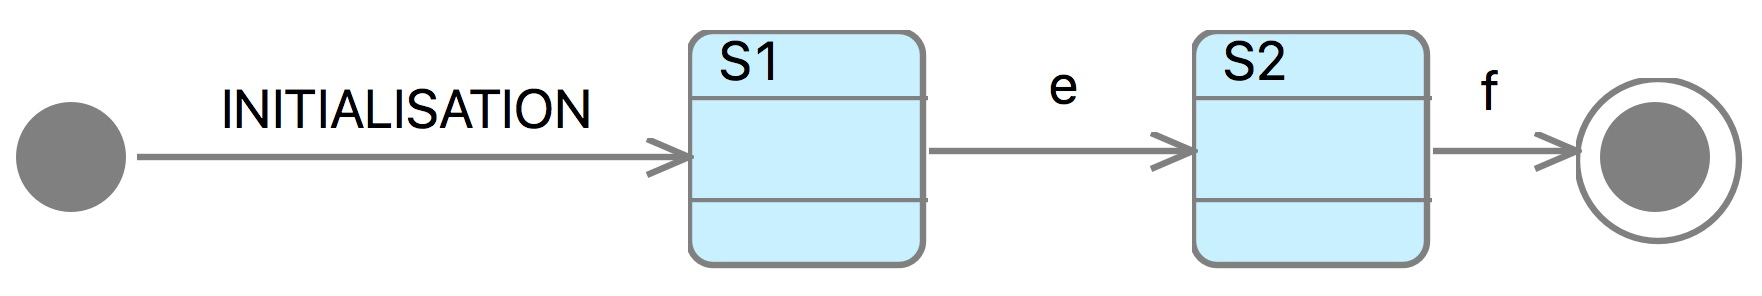
\includegraphics[width=0.6\textwidth]{figures/iumlb-SM}
% 	\caption{An example \UMLB state-machine}
% 	\label{fig:iumlb-sm}
% 	\vspace{-.5cm}
% \end{figure}

Each state is encoded as a boolean variable and the current state is indicated by one of the boolean variables being set to |TRUE|. 
An invariant ensures that only one state is set to |TRUE| at a time.
%The state-machine, is initialised by setting one state variable to |TRUE| and all others to |FALSE|.
Events change the values of state variables to move the |TRUE| value according to the transitions in the state-machine.  
% The \EventB translation%
% %
% \footnote{%
%   Here, $\mathrm{partition(S, T1, T2, \ldots)}$ means the set $S$ is partitioned into disjoint (sub-)sets $T1, T2, \ldots$.
% that cover $S$} 
% of the state-machine in Figure~\ref{fig:iumlb-sm} can be seen in Listing~\ref{lst:eventb-sm}.
% \UMLB also provides the option of an alternative translation with a single state variable ranging over an enumerated type of states, however, the boolean representation of each state is more natural for a user to reference in \SCXML guards and actions.
	
While the \UMLB translation deals with the basic data formalisation of state-machines it differs 
significantly from the semantics discussed in this manuscript. 
\UMLB adopts \EventB's simple guarded action semantics and does not have a concept of triggers and run-to-completion.
Here we make use of \UMLB's state-machine translation but provide a completely different semantic by generating a behaviour into the underlying \EventB events that are linked to the generated \UMLB transitions.
% \begin{lstlisting}[caption={Translation of the state-machine in Fig.~\ref{fig:iumlb-sm}},label={lst:eventb-sm}, language=Event-B, escapechar=|, frame=single]
% variables S1 S2
% invariants 
% 	TRUE !: {S1, S2} => partition({TRUE}, {S1}/\{TRUE}, {S2}/\{TRUE})
% events
%     INITIALISATION: begin S1, S2 := TRUE, FALSE end
%     e: when S1 = TRUE then S1, S2 ≔ FALSE, TRUE  end
%     f: when S2 = TRUE then S2 := FALSE end
% end
% \end{lstlisting}
%%% Local Variables:
%%% mode: latex
%%% TeX-master: "../main"
%%% End:

% !TEX root = ../main.tex

\subsection{SCXML}
\label{sec:scxml}

\SCXML is a modelling language based on Harel statecharts with facilities for adding data elements that are manipulated by transition actions and used in conditions for their firing. \SCXML follows the usual `run to completion' semantics of such statechart languages, where trigger events\footnote{In \SCXML the triggers are called `events', however, we refer to them as `triggers' to avoid confusion with \EventB} may be needed to enable transitions. Trigger events are queued when they are raised, and then one is de-queued and consumed by firing all the transitions that it enables, followed by any (un-triggered) transitions that then become enabled due to the change of state caused by the initial transition firing. This is repeated until no transitions are enabled, and then the next trigger is de-queued and consumed. There are two kinds of triggers: internal triggers are raised by transitions and external triggers are raised by the environment (spontaneously as far as our model is concerned). An external trigger may only be consumed when the internal trigger queue has been emptied. 

\begin{lstlisting}[caption=Pseudocode for 'run to completion',label={lst:scxml-r2c}, frame=single]
while running:
	while completion = false
		if untriggered_enabled
			execute(untriggered())
		elseif IQ /= {}
			execute(internal(IQ.dequeue)) 
		else
			completion = true
		endif
	endwhile
	if EQ /= {}
		execute(EQ.dequeue) 
		completion = false
	endif
endwhile 
\end{lstlisting}

Listing~\ref{lst:scxml-r2c} shows a pseudocode representation of the run to completion semantics as defined within the latest W3C recommendation document~\cite{scxmlwebsite}. Here IQ and EQ are the triggers present in the internal and external queues respectively. We adopt the commonly used terminology where a single transition is called a \emph{micro-step} and a complete run (between de-queueing external triggers) is referred to as a \emph{macro-step}.

%%% Local Variables: 
%%% mode: latex
%%% TeX-master: "../main.tex"
%%% End: 


%%% Local Variables:
%%% mode: latex
%%% TeX-master: "../main"
%%% End:


\section{Formalisation using Contexts/Machines vs Theories}
\label{sec:formalisation}

In this section, we present an attempt to formalise the semantics of statemachines using theories, in comparison with the contexts/machines as in~\cite{DBLP:conf/ictac/WrightHSB23}. Figure~\ref{fig:scxml-thy-form} show our strategy for developing a semantics of statecharts using theories.
\begin{figure}
    \centering
    \includegraphics[width=0.6\textwidth]{figures/SCXML_thy_form.jpg}
    \caption{Formalisation of statemachines: contexts/machines vs theories}
    \label{fig:scxml-thy-form}
\end{figure}

\subsection{Formalisation of \texttt{closure}}
In~\cite{DBLP:conf/ictac/WrightHSB23}, the (irreflexive) transitive closure is formalised as a constant with an axiom defining its value. Various theorems capturing the properties of |closure| are derived from the axiom. Here |STATE| is a carrier set defining the set of states in the statemachines.
\begin{EventBcode}
constants closure
axioms
	@def-closure: closure = (λ r · r ∈ STATE ↔ STATE ∣ inter({p ∣ r ⊆ p ∧ p;p ⊆ p}))
	theorem @typeof-closure: closure ∈ (STATE ↔ STATE) → (STATE ↔ STATE)	
	theorem @closure_strengthen: ∀ r· r ⊆ closure(r)
	theorem @closure_transitivity: ∀ r·closure(r);closure(r) ⊆ closure(r) 	
	theorem @closure_minimal: ∀ r·(∀ p· r⊆p ∧ p;p⊆p ⇒ closure(r)⊆p)
\end{EventBcode}
Using the Theory plug-in, |closure| is defined as an operator in a theory for type parameter |S|. This operator is polymorphic with respect to this type parameter and hence can be utilised in different contexts (compared with the constant defined in the context for a specific |STATE| set).
\begin{center}
    \includegraphics[width=0.9\textwidth]{figures/cl_thy.jpg}
\end{center}

\subsection{Formalisation of \texttt{tree}}
Using context, the definition of trees is defined as a constant |Tree| with its value defined using set comprehension and utilising transitive closure. In this definition, |Sts| represents the set of nodes in a tree, |rt| represents the root of the tree, and |prn| is the parent relationship of the tree.
\begin{EventBcode}
axioms @def-Tree: Tree = {Sts ↦ rt ↦ prn ∣
			Sts ⊆ STATE ∧ rt ∈ Sts ∧ prn ∈ Sts ∖ {rt} → Sts ∧ (∀ n · n ∈ Sts ∖ {rt} ⇒ rt ∈ cl(prn)[{n}])}
\end{EventBcode}
Following the EB4EB framework~\cite{DBLP:conf/nfm/RiviereSAD23}, we formalise tree as a datatype with a well-definedness operator. The datatype is polymorphic with a type parameter |NODE| and  operator |TreeWD| stating similar conditions in the axiom |@def-Tree|.
\begin{center}
    \includegraphics[width=0.7\textwidth]{figures/tree_thy.jpg}
\end{center}

\subsection{Formalisation of the Statechart Syntactical Elements}
The syntactical elements of the statecharts are captured in three contexts to introduce the different aspects gradually: (1) tree-shape structure (2) parallel regions, and (3) transformations (an abstraction of transitions between states, including enabling, entering, and exiting states for each transformation). We will not present the details of the formalisation here, but refer the readers to~\cite{DBLP:conf/ictac/WrightHSB23}.
\begin{figure}[!h]
    \centering
    \includegraphics[width=0.5\textwidth]{figures/sc_data_thy.jpg}
    \caption{Statechart datatype}
    \label{fig:sc-data-thy}
\end{figure}
Using the Theory plugin, we define the |STATECHART| datatype as in Figure~\ref{fig:sc-data-thy}. Notice that we decide to define the |STATECHART| datatype all at once rather than gradually introducing its aspects. Datatypes in the Theory plugin are closed and hence cannot be extended. An example is the use of the |Tree| datatype for part of the |STATECHART| datatype resulting in a ``nesting'' effect. This result in the following operators to define the well-definedness for |Regions| of a statechart. In order to get to the states of a statechart |st|, one need to use |States(Tree(st))| due to this nesting effect.
\begin{center}
    \includegraphics[width=0.9\textwidth]{figures/regions_wd_thy.jpg}
\end{center}

\subsection{Formalisation of the Statechart Semantical Elements}
In~\cite{DBLP:conf/ictac/WrightHSB23}, the semantical elements of the statecharts are captured in a machine with a variable representing the active states of the statechart. Invariants capture properties, such as there is always an active state and if a child state is active then its parent state must be active.

Using the Theory plugin, we define a datatype |ACTIVE_STATECHART| for this purpose (we omit some details for spacing reason). This datatype wraps the |STATECHART| datatype together with the active states. The well-definedness operator |ActiveStatechartWD| captures the properties that we want to impose on the statechart semantics.
\begin{center}
    \includegraphics[width=1.0\textwidth]{figures/asc_thy.jpg}
\end{center}
We define the |transformation| operator and state the following theorem (to be proved). The theorem says that any transformation of an active statechart preserves the well-definedness of the active statechart.
\begin{center}
    \includegraphics[width=1.0\textwidth]{figures/asc_wd_thy.jpg}
\end{center}

\section{Conclusion}

In conclusion ...

% ---- Bibliography ----
\bibliographystyle{splncs04}
\bibliography{paper}
\end{document}
